\section{Объект управления}

Основными объектами управления рассматриваемого в данной работе метода являются механизмы, роботы, манипуляторы, кинематика которых описываются простыми кинематическими цепями.

Типичным представителем таких механизмов являются роботы-манипуляторы.

\begin{center}
  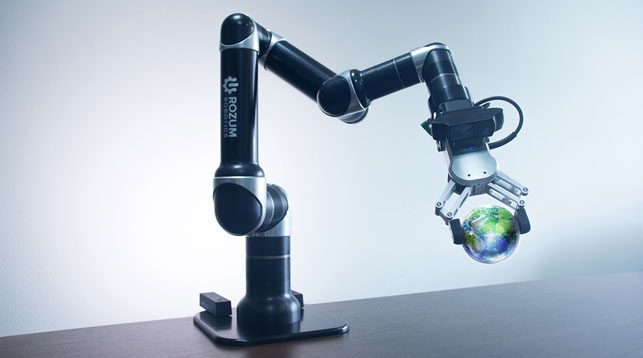
\includegraphics[width=0.6\textwidth,height=0.6\textheight,keepaspectratio]{manip1.jpg}
  \captionof{figure}{Манипулятор на поворотных звеньях. (Rozum Robotics)}
  \label{}
\end{center}

\begin{center}
  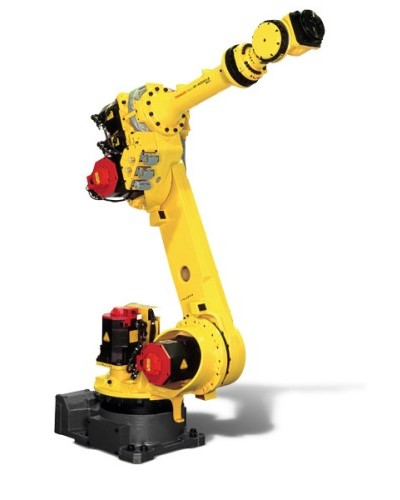
\includegraphics[width=0.6\textwidth,height=0.6\textheight,keepaspectratio]{manip2.jpg}
  \captionof{figure}{Манипулятор на поворотных звеньях (FANUC R-1000iA80H)}
  \label{}
\end{center}

Управление положением схвата первично для таких изделий. Зачастую роботы манипуляторы имеют избыточную кинематику, что ставит вопрос о поиске управления, исключающего коллизии и сингулярные состояния.

Другой тип рассматриваемых объектов управления, позиционеры, сочитающие линейные и вращающие звенья:

\begin{center}
  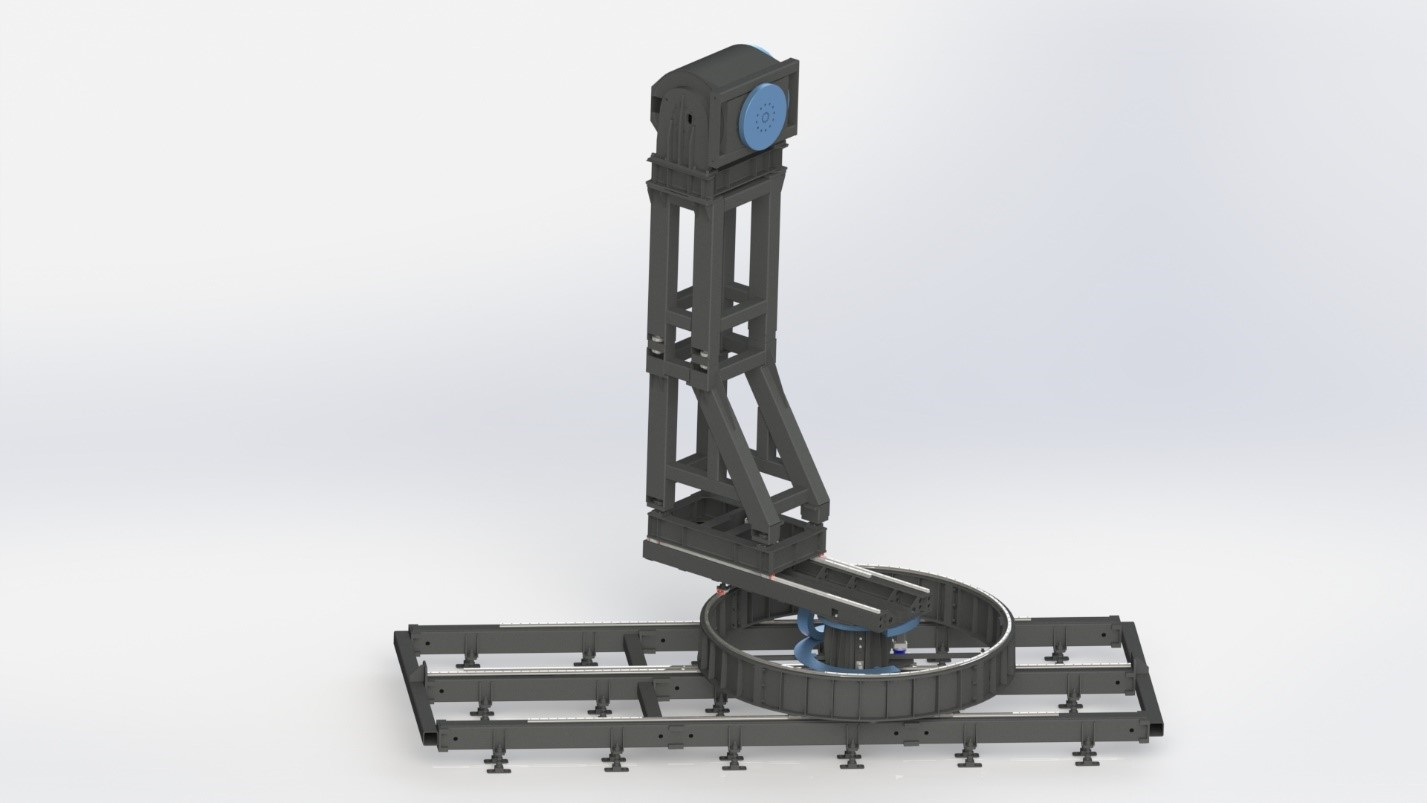
\includegraphics[width=0.6\textwidth,height=0.6\textheight,keepaspectratio]{actexample.jpg}
  \captionof{figure}{Позиционер с линейными и поворотными звеньями (Radioline PSR)}
  \label{}
\end{center}

Характеризуются меньшей избыточностью кинематики, имеют высокую жесткость и точность позиционирования.

В качестве перспективного направления развития метода рассматривается управление манипуляторами мобильных платформ (колёсных, шагающих, летающих).

\begin{center}
  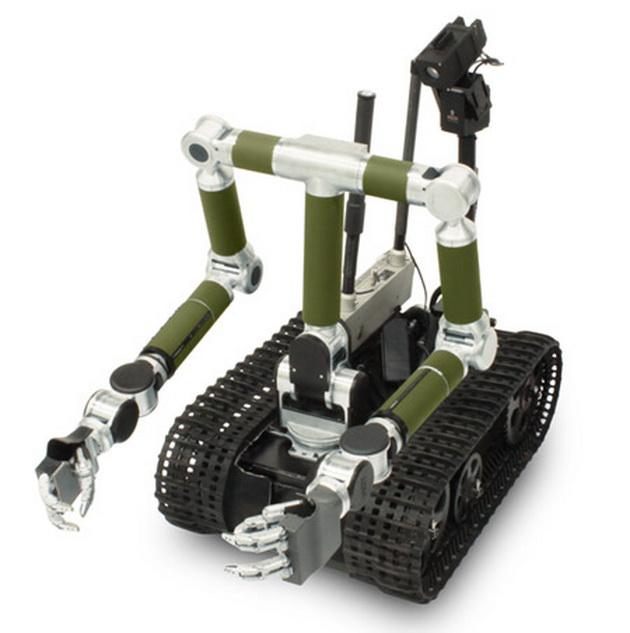
\includegraphics[width=0.6\textwidth,height=0.6\textheight,keepaspectratio]{mobile.jpg}
  \captionof{figure}{Мобильная платформа с манипулятором.}
  \label{}
\end{center}

\begin{center}
  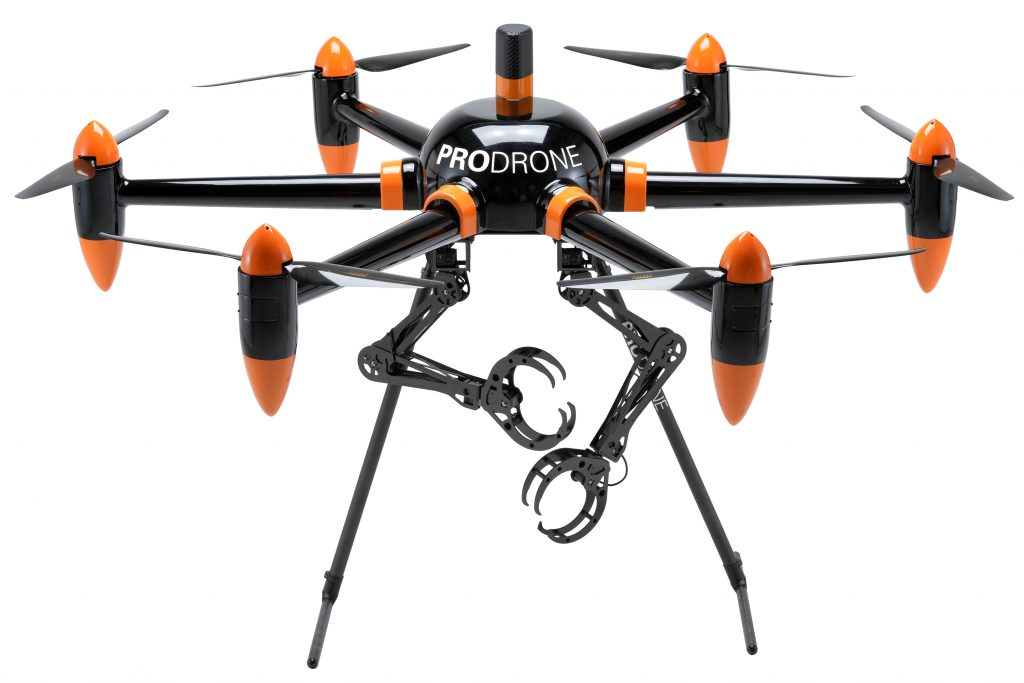
\includegraphics[width=0.6\textwidth,height=0.6\textheight,keepaspectratio]{fly.jpg}
  \captionof{figure}{Летающая платформа с манипулятором.}
  \label{}
\end{center}

\begin{center}
  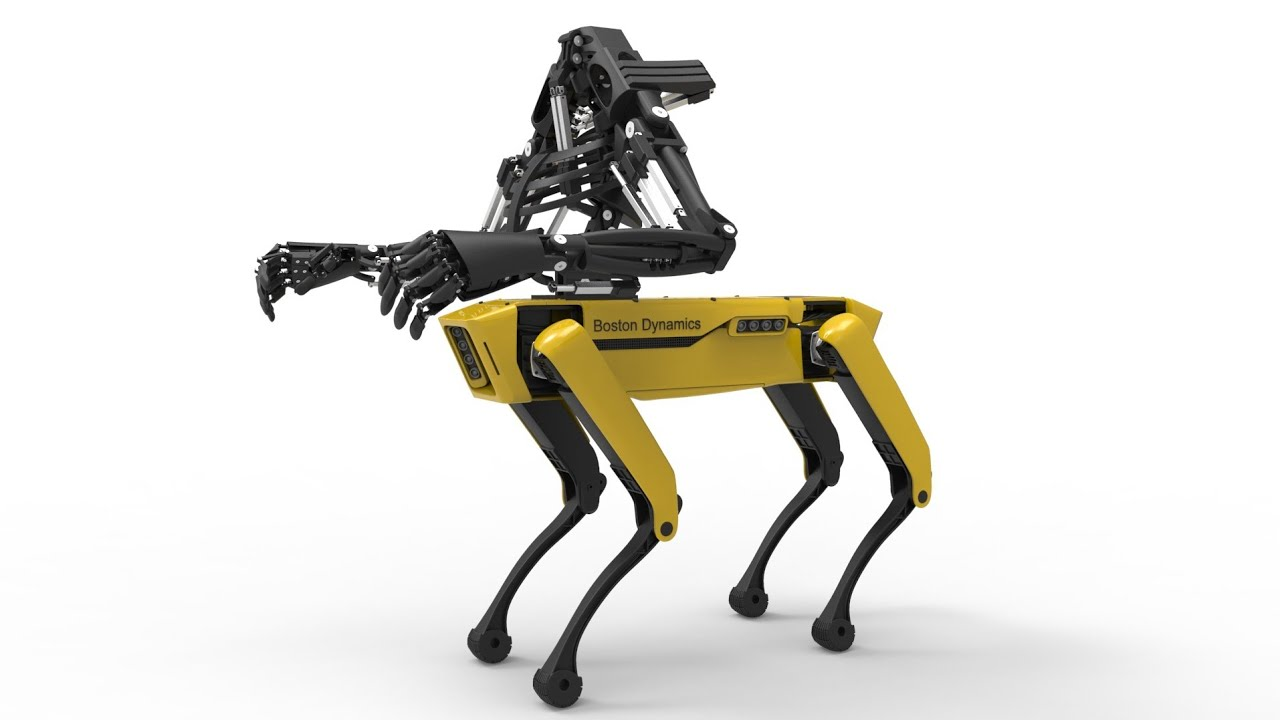
\includegraphics[width=0.6\textwidth,height=0.6\textheight,keepaspectratio]{centaurus.jpg}
  \captionof{figure}{Шагающая платформа с манипулятором.}
  \label{}
\end{center}

В качестве перспективного направления развития метода также рассматривается управление сложными схватами.

\begin{center}
  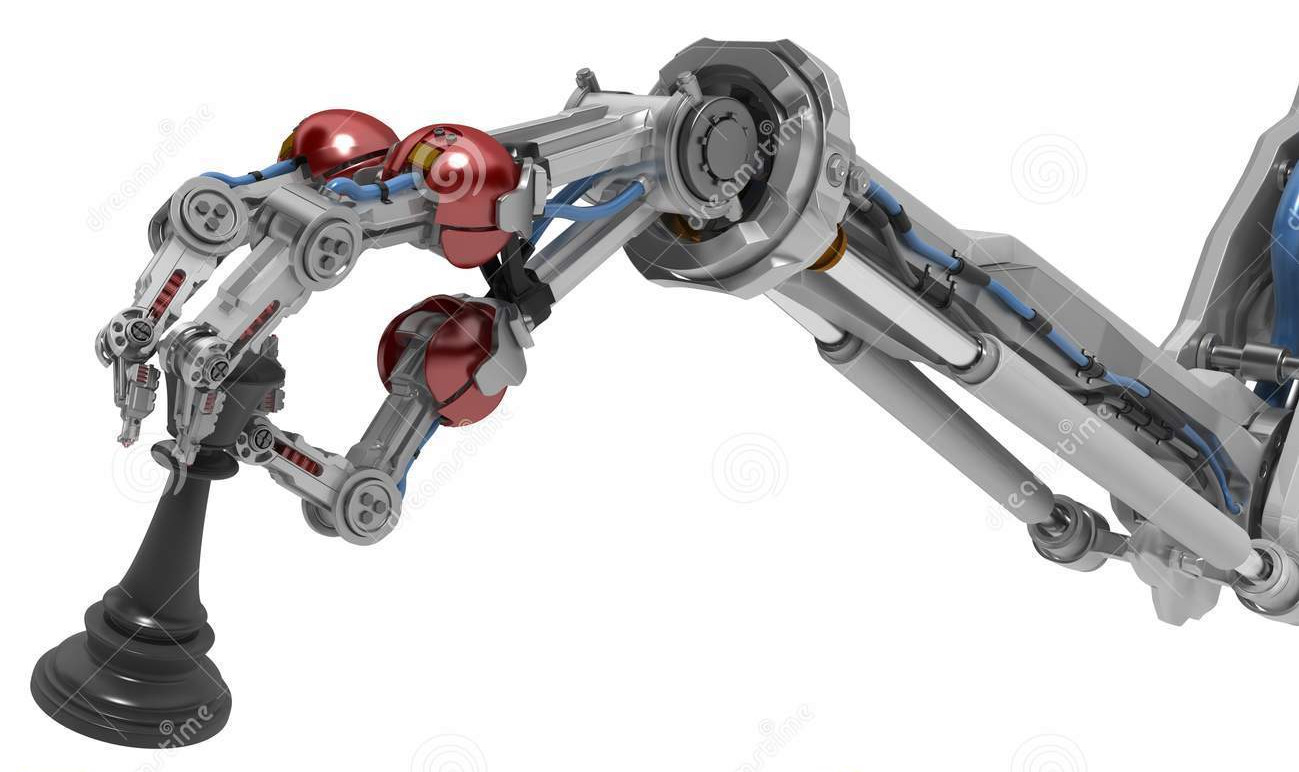
\includegraphics[width=0.6\textwidth,height=0.6\textheight,keepaspectratio]{arm.jpg}
  \captionof{figure}{Пример сложного манипулятора.}
  \label{}
\end{center}

Эти объекты требуют синхронного многокоординатного управления положением, которое в рамках рассматриваемого метода осуществляется через построение следящей системы с модельной уставкой положения выходного звена/звеньев.

